\documentclass[a4paper,10pt]{article}
\usepackage[utf8]{inputenc}
\setcounter{tocdepth}{2} %Only show sections and subsections in toc.

\usepackage{colortbl}
\usepackage{siunitx} %Package for SI units
\sisetup{per-mode=fraction}

\usepackage{textcomp} %Vertically centered tilde (~)
\usepackage{amsmath}
\usepackage{graphicx}
\usepackage{standalone}

\usepackage[font={footnotesize}]{caption}
\usepackage[font={footnotesize}]{subcaption}

\usepackage[hidelinks]{hyperref}
%\hypersetup{
%    colorlinks = false,
%    linkbordercolor = {white},
%}


%\hypersetup{
 %   colorlinks,
 %   linkcolor={red!50!black},
 %   citecolor={blue!50!black},
 %   urlcolor={blue!80!black}
%}

\usepackage{float}
\usepackage[procnames]{listings}
\usepackage{epstopdf} %Convert EPS files to PDF format
\usepackage{pdfpages} %Utility to include pdf documents into the report, used to include datasheets in appendices.

\usepackage{tikz} 			%Utility to draw nice figures
\usetikzlibrary{shapes.geometric, arrows}
\usepackage{standalone}
\usepackage{circuitikz} 	%Utility to draw circuits in tikz

\usepackage[disable]{todonotes}
\usepackage{listings}
\usepackage{multirow}


\usepackage{url}
\renewcommand{\UrlFont}{\large\tt}

\usepackage{chngcntr} %Change the counters of objects. Used to make figure/table and equation counting specific to the section they are in.
\counterwithin{figure}{section}
\counterwithin{equation}{section}

%Make counter of listings specific to sections
\AtBeginDocument{%
  \counterwithin*{lstlisting}{section}
  \renewcommand{\thelstlisting}{%
    \ifnum\value{subsection}=0
      \thesection.\arabic{lstlisting}%
    \else
      \ifnum\value{subsubsection}=0
        \thesection.\arabic{lstlisting}%
      \else
        \thesection.\arabic{lstlisting}%
      \fi
    \fi
  }%
}

%\usepackage[inner=2cm,outer=4cm]{geometry}



\setlength{\parindent}{0pt}

\title{Electronics - 1. Semester Project}
\author{Thomas S�ndergaard Christensen, Mikkel 
Skarup Jaedicke, Martin Br'chner Andersen}
\date{dd/mm/2016}


\begin{document}
%!TEX root = ../main.tex
\begin{titlepage}
%\newgeometry{left=3cm,right=3cm}
\begin{center}

\textsc{\LARGE University of Southern Denmark}\\[1.5cm]
\textsc{\Large MSc in Engineering - Electronics}\\
\textsc{\large 2. Semester Project}\\[0.5cm]

\vfill
\vspace{3cm}
\hrule ~\\[0.3cm]
{ \LARGE \bfseries We need a title\\[0.4cm] }
\hrule ~\\[1.5cm]

\vfill

%\includegraphics[width=0.3\textwidth]{graphics/sdu_logo}
\vspace{7cm}
% Author and supervisor
\begin{minipage}[t]{.49\textwidth}
\begin{flushleft} \large
\textbf{Authors:}\\
230390 Martin Brøchner Andersen\\
430583 Catalin Ionut Ntemkas\\
030192 Mikkel Skaarup Jaedicke\\
100589 Thomas S. Christensen
\end{flushleft}
\end{minipage}
\begin{minipage}[t]{.49\textwidth}
\begin{flushright} \large
\textbf{Supervisors:} \\
Leon xxxxx
\end{flushright}
\end{minipage}

\vspace{1cm}
Date: xx-xx-2016

\vspace{1cm}

\end{center}
%\restoregeometry
\end{titlepage}
\newpage
\pagenumbering{Roman}
%!TEX root = ../main.tex
\section*{Preface}
\addcontentsline{toc}{section}{Preface}

\section*{Acknowledgment}
\addcontentsline{toc}{section}{Acknowledgment}
This project would not have been possible without the invaluable assistance and patience of our supervisor. 
A Tremendous thank you to Leon Bonde Larsen.
The process was simplified by Assistant Professor Kjeld Jensen from which the sensory equipment used in the report was supplied.
\thomas{Rewritten - needs a bit more?}
\martin{Who else should we thank? Viking Pizza?}
\mikkel{NEW URL}
\vspace{5cm}
\begin{center}
	\begin{minipage}[t]{.55\textwidth}\large
		\begin{center}
		Catalin Ionut Ntemkas\\
		\vspace{1cm}
		\hrule
		\vspace{0.5cm}
		Martin Brøchner Andersen\\
		\vspace{1cm}
		\hrule
		\vspace{0.5cm}
		Mikkel Skaarup Jaedicke\\
		\vspace{1cm}
		\hrule
		\vspace{0.5cm}
		Thomas Søndergaard Christensen
		\vspace{1cm}
		\hrule
		\end{center} 
	\end{minipage}
\end{center}

\vspace{1.2cm}
  \begin{center}
    \textsl{The report, source code, data, plotting script and simulations can be found at:}  
    \end{center}
    \vspace{-5pt}
    \begin{center}
	\renewcommand{\UrlFont}{\color{black}\normalsize\tt}
    \url{github.com/mikkeljae/SEM1PRO_ELECTRONICS}
   \end{center}
\newpage

\section*{Abstract}
\addcontentsline{toc}{section}{Abstract}
A go-kart has been supplied as a development platform for student projects at University of Southern Denmark.
In the interest of enabling more complex projects, a unified data collection system is necessary.
This is developed throughout this report. 
An analysis is done to determine the requirements of such a system.
It was found that a two-part network is suitable for this application.
The two parts are a CAN network and an ad-hoc WiFi network.
A custom protocol for use on CAN, GoCAN, is developed.
GoCAN supports up to 16 sensors from which data can be monitored on a remote monitoring station using the WiFi connection.
The system was only partially implemented since a connection between the CAN network and Linux was not achieved.
\thomas{Rewritten}
\newpage
\tableofcontents
\newpage
\listoftodos
%\listoftables
\clearpage
\newpage
\pagenumbering{arabic}
%!TEX root = ../main.tex
\section{Monitoring of sensor data on the SDU go-kart.}
This project aims to produce a tool for developing, evaluating and testing hardware for the SDU go-kart.
Movement of the go-kart should be monitored to enable evaluation of the performance of the go-kart.
The control variables and currents of the inverter should be monitored in order to help develop new hardware or evaluate existing hardware.
A basic use case diagram showing the functionality of the system can be seen in figure \ref{fig:use_cases}.
The use case narratives are shown in tables \ref{tab:use_monitor} to \ref{tab:use_read_log}.
\begin{figure}[h]
 	\centering
    \includegraphics[width=0.8\textwidth]{graphics/use_cases}
    \caption{Use case diagram for the system.}
    \label{fig:use_cases}
\end{figure}


\begin{table}[]
\centering
\caption{Usecase narrative for monitor live data from go-kart.}
\label{tab:use_monitor}
\begin{tabular}{| r | p{6 cm} |}
\hline
\textbf{Use case:}                        & Monitor live data from go-kart                  \\ 
\textbf{Actors:}                          & Engineer                                        \\
\textbf{Purpose:}                         & Monitor live data from go-kart                  \\
\textbf{Overview:}                        & The engineer starts the system. The system will begin collecting data on the go-kart and transfer them to a stationary computer. The computer will present data to the engineer on a GUI. \\
\textbf{Type:}                            & Essential                                       \\
\textbf{Preconditions:}                   & -                                               \\
\textbf{Postconditions:}                  & System transfers data from go-kart sensors to a stationary computer, showing data in a GUI.                                                                                            \\
\textbf{Special requirements:}            & -                                               \\ \hline 
\multicolumn{1}{|c|}{\textbf{Actor action}} & \multicolumn{1}{c|}{\textbf{System response}}\\
\multicolumn{1}{|l|}{1. Start system}       & \begin{tabular}[c]{@{}l@{}}2. Start collecting data\\ 3. Transfer data to stationary computer\\ 4. Present data in GUI\end{tabular}                                              \\ \hline
\multicolumn{2}{|c|}{\textbf{Alternative flow of events}}                                   \\
\multicolumn{2}{|p{12 cm}|}{Any line: User can stop the system at any point in time.}              \\ \hline                                                                                                                                    
\end{tabular}
\end{table}


\begin{table}[]
\centering
\caption{Usecase narrative for log go-kart data.}
\label{tab:use_log}
\begin{tabular}{| r | p{6 cm} |}
\hline
\textbf{Use case:}                        & Log go-kart data            			        \\ 
\textbf{Actors:}                          & Engineer                                        \\
\textbf{Purpose:}                         & Log go-kart data                 				\\
\textbf{Overview:}                        & After startup the system will log the collected go-kart data on xx  \\
\textbf{Type:}                            & Essential                                       \\
\textbf{Preconditions:}                   & System is running and collecting go-kart data   \\
\textbf{Postconditions:}                  & System logs collected go-kart data.      		\\
\textbf{Special requirements:}            & -                                               \\ \hline 
\multicolumn{1}{|c|}{\textbf{Actor action}} & \multicolumn{1}{c|}{\textbf{System response}} \\
\multicolumn{1}{|l|}{}       & \begin{tabular}[c]{@{}l@{}}1. Log collected data\end{tabular}\\ \hline
\multicolumn{2}{|c|}{\textbf{Alternative flow of events}}                                   \\
\multicolumn{2}{|p{12 cm}|}{Any line: User can stop the logging	 at any point in time.}         \\ \hline                                                                                                                                    
\end{tabular}
\end{table}



\begin{table}[]
\centering
\caption{Usecase narrative for read logged data.}
\label{tab:use_read_log}
\begin{tabular}{| r | p{6 cm} |}
\hline
\textbf{Use case:}                        & Read logged data  			                    \\ 
\textbf{Actors:}                          & Engineer                                        \\
\textbf{Purpose:}                         & Monitor live data from go-kart                  \\
\textbf{Overview:}                        & The engineer will ask the system for the logged data. The system will transfer the logged data to a stationary computer \\
\textbf{Type:}                            & Essential                                       \\
\textbf{Preconditions:}                   & Data is logged in logfile on xx                 \\
\textbf{Postconditions:}                  & The log file is on the stationary computer                                                                                      \\
\textbf{Special requirements:}            & -                                               \\ \hline 
\multicolumn{1}{|c|}{\textbf{Actor action}} & \multicolumn{1}{c|}{\textbf{System response}}\\
\multicolumn{1}{|l|}{1. Ask for log file}       & \begin{tabular}[c]{@{}l@{}}2. Transfer logged data to statinary computer\\ 3. Save data to log file on stationary computer\end{tabular}                                              \\ \hline
\multicolumn{2}{|c|}{\textbf{Alternative flow of events}}                                   \\
\multicolumn{2}{|p{12 cm}|}{Any line: If connection is lost the system should detect it and mark the trasferred log file as invalid}              \\ \hline                                                                                                                                    
\end{tabular}
\end{table}



%Relavant control variables should be controllable, while driving allowing for efficient testing of controllers.
To achieve this, data should be collected on a computer on the go-kart and sent to a stationary computer.

%\subsection{What is the role of transferring go-kart data to and from a stationary computer?}
%To let an engineer or a mechanic monitor the status of the go-kart.

%Movement data could be usefull for testing new hardware, improving existing hardware and evaluation the drivers performance. 
%Data about battery status, currents, motortemperature is usefull for safety procedures.
%Data from the SEVCON xxx inverter or other inverters on the go-kart could be used for tuning parameters, evaluation performance and safety measures.
%On the basis of this data it should be possibly to change configuration parameters on the SEVCON xxx while driving the go-kart.

\subsection{What is the role of the stationary computer?}
The stationary computer should be responsible of the transmission of relevant go-kart data to and from the "on-board" computer.
The received data should be presented to the user in a SCADA system.

\subsubsection*{What data and sensors would be interesting to monitor?}
Data from IMU, GPS and encoders would be necessary to monitor the movement of the go-kart.
Data from the SEVCON xxx gives information about about battery status, currents, motortemperature.
%Temperature of tyres, speed of front wheels, possibility to control or at least moniter stearing and brake.
It should be possible to get data from a new inverter, that is not yet made. 

\subsubsection*{What kind is the stationary computer?}
It should be possible for different personnel to monitor the go-kart data therefore the statinonary computer should just be general purpose computer running (linux?).

\subsubsection*{What kind of communication is needed to transfer data between the go-kart computer and the stationary computer?}
As it should be possibly to monitor data while the go-kart is driving the connection clearly needs to be wireless with a range allowing for driving on a typical racing track. 
As all data is used by humans the propagation delay of the connection is not required to be very low.

\subsubsection*{How should data on the stationary computer be presented?}
As live data should be easy to read? ("overskue" in danish) there needs to be a GUI or at least a UI that will present the user with easy readable data. SCADA SYSTEM!?!?!
Changing of parameters on the go-kart should also be in the UI in order useable by others than the developers.

\subsection{What is the role of the computer on the go-kart?}
The "onboard" computer needs to handle the collection
of data from different sensors (data producers).
This computer will also handle the transmission of data to the stationary 
computer.
%There are tasks that need to be handled locally fx strict safety measures (and future things fx localisation) that requires a miminum delay. 
Storing of data with a 
The computer needs also to store data locally in order to avoid data loss if the wireless connection is lost.

\subsubsection*{How is local data transmission handled?}
All data should be collected locally on the "on-board" computer to transmit it to the stationary computer.
Local data collection should be "fast" and "reliable" for local safety measures to function properly.
It should be possibly to collect data from and transmit data to at least the 
aforementioned IMU, GPS and SEVCON xx with the possibility of adding additional 
data producers.

\subsubsection*{What kind is the "on-board" computer?}
The computer should be a small embedded platform in order to mount it physcically on the go-kart.
It should be able to handle all "on-board" tasks.

\subsubsection*{How should local data storage be realised?}
Data should be stored directly on nonvolatile memory to be able retrieve data after shutdown.
Data integrity checks is needed to ensure proper data logging.
%Correct data logging should be realised to ensure validity of data. 


\newpage
\section{System requirements}

\subsection{Actors}
The only actor on the system is an engineer.

\subsection{Interfaces}
\begin{itemize}
\item Wifi, for data transfer between go-kart and stationary computer.
\item CAN bus, for local network.
\item CanOpen, for interfacing the Sevcon.
\item USB, for GPS and IMU.
\item ??, for SD card connection.
\item Powersupply, for Zybo boards.
\end{itemize}

\subsection{Functional requirements}
The system: 
\begin{itemize}
\item Reads data from sensors.
\item Reads data from Sevcon.
\item Transfers data to stationary computer using Wifi.
\item Presents data to the user.
\item Logs sensordata to SD card.
\item Read data from SD card.
\item Timestamps all data. 
\end{itemize}

\subsection{Operational requirements}
The system monitors go-kart data.% when engineer starts the system by powering it on.

\subsection{Quality of service requirements}
\begin{itemize}
\item IMU data must be sampled with xx Hz.
\item GPS data must be sampled with zz Hz.
\item Data logging with qq Hz.??
\end{itemize}

\subsection{Parametric requirements}
Wifi range must be greater than xx meters.

\subsection{Design requirements}
The system:
\begin{itemize}
\item must be scalable to at least 16 sensors/nodes.
\item must be modular to allow easy integration of new sensors/nodes.
\item must be functional if one or more sensors/nodes stop working.	 
\end{itemize}



\newpage
\section{Further ivestigation}

\subsection{Parameters of Interest}
\label{sec:parameters}
In developing new hardware or evaluating current hardware, it is necessary to be able to monitor a range of parameters.
This section will investigate what parameters need to be logged in order to provide a useful and complete logging of the behaviour of the go-kart.
The parameters in question fall into three categories; Physical parameters, electrical parameters and mechanical parameters.
These will be dealt with in turn in the following sections
\paragraph*{Physical Parameters}
This category comprises all information about the motion of the go-kart.
\begin{itemize}
	\item \textbf{Position, Absolute:} Providing a means to record the absolute position of the go-kart is a useful feature in certain fields.
	Especially any form of localisation and pathfinding will be able to put this information to use.
	The absolute position of the go-kart can be recorded using a GPS module or possibly by using a known starting coordinate and information about the relative movement of the go-kart.
	\item \textbf{Position, Relative:} The relative position of the kart can be, as just mentioned, used to infer the absolute position of the go-kart.
	Additionally it can provide a means to analyze a drivers performance on the track or detect drift while cornoring.
	The relative position includes both translational, as well as rotational information.
	This information can be gathered using an inertial measurement unit (IMU).
	An IMU is a compound device, comprising of an accelerometer and a gyroscope and, in some cases, a magnetometer.
	\item \textbf{Velocity:} The velocity of the go-kart is key in optimising lap-times, clearly, it is desirable to monitor this parameter.
	It can be extracted by reading the motor encoders.
	However, the driving wheels are prone to slippage when cornoring, this would give an inaccurate reading of the actual velocity of the go-kart.
	Instead, a simple encoder can be mounted on either one, or both of the front wheels as these are freerunning and independent.
	Once the rotational speed of the axle is known, the velocity of the go-kart can be infered using the tyre diameter.
	\item \textbf{Acceleration:} It may be of interest to monitor the forces exerted on the go-kart, or, its acceleration, as it drives on the track.
	This information is already provided by the accelerometer in the IMU mentioned above and as such provides no additional complication.
\end{itemize}
Three sensors are mentioned in this section.
A GPS, an IMU and an encoder.
In order to limit the scope of the project only the GPS and the IMU will be implemented.
\paragraph*{Electrical Parameters}
This category comprises all information about the electrical aspects of the go-kart.
\begin{itemize}
	\item \textbf{Motor Currents:} Providing a means of monitoring the currents flowing through the motor allows the user to calculate the torque exerted by the motor as well as the current power draw of the motor.
	Knowing the currents could also prove an invaluable debugging tool when developing a new inverter for the go-kart.
	\item \textbf{Throttle Position:} The throttle on the go-kart is connected to a potentiometer.
	Measuring the voltage output of this potentiometer provides a simple way of monitoring the position of the throttle.
	\item \textbf{Desired Currents:} Based on the current throttle position a set of desired currents are calculated.
	Monitoring these allows spotting any discrepancies between the desired and the actual currents.
	\item \textbf{Duty Cycles:}
	\item \textbf{Battery Voltage:} As the go-kart is electrical, naturally, it has a battery.
	Monitoring the current battery status could give the user an indication of how much driving time is left, or how long until the batteries are recharged afterwards.
	\item \textbf{Motor Angle:} Knowing the angle of the motor at all times gives a means of more accurately calculate the currents at specific times.
	Additionally, it can be used in Clarke-Parke transformations, again, providing information in debugging an inverter in development.
\end{itemize}
These parameters are all available from the sevcon gen4 motor controller mounted on the go-kart.
This controller has a CANopen interface from which this data can be extracted.
Any users who wish to add their own inverter will simply need to obey the API stated by the sevcon gen4 CANopen interface in order to correctly log the data.
\paragraph*{Mechanical Information}
This category comprises all information about the mechanical aspects of the go-kart.
\begin{itemize}
	\item \textbf{Steering Wheel Angle:} Monitoring the angle of the steering wheel allows analysing the performance of the driver.
	In addition it opens up for the possibility of mechanical control of the go-kart.
	Similarly to monitoring the velocity, the steering wheel angle can be monitored by adding an encoder to the steering column.
	\item \textbf{Braking Pedal Position:} The braking system on the go-kart is similar to that of an ordinary car.
	The braking disc is mounted on the driving axle and the braking calibers connected to the brake pedal by a series of oil-filled hoses.
	Monitoring its actuation allows analysing the performance of the driver and as mentioned above, may potentially allow for mechanical control of the go-kart
\end{itemize}
As both of these parameters would require mechanical changes to the go-kart, they are beyond the scope of this project and as such will not be implemented.
\subsubsection*{Conclusion}
In this section a multitude of different parameters have been discussed.
Most of them can be logged using just three components; a Sevcon Gen4 motor controller, an IMU and a GPS.
These are the three components from which data logging will be implemented throughout this project.
This provides a solid platform to prove the concept and additional sensory equipment can be added at a later date, should it be required.

\subsection{Hardware for Monitoring Parameters}
In section \ref{sec:parameter} an overview of the different parameters that may be of interest for logging is given.
It was concluded that three components would suffice as a proof of concept; the Sevcon Gen4 motor controller, an IMU and a GPS.
This section will explore in more detail what requirements and communication schemes exists for each of the components.

\subsubsection*{Sevcon Gen4 Motor Controller}

\subsubsection*{Inertial Measurement Unit (IMU)}
IMU's, generally, exist in two versions.
A 6D and a 9D version.
Both include an accelerometer and a gyroscope.
In addition to these the 9D IMU includes a magnetometer, enabling measurement of absolute direction, as opposed to the relative measurement of direction granted by the magnetometer.
The requirement in terms of each of these parts is given as:
\begin{itemize}
	\item \textbf{Accelerometer [\si{\metre\per\second^2}]:} As the name implies, the accelerometer measures accelerations.
	That is, when the component changes speed or direction the force exerted on the accelerometer is measured.
	Professional drivers using professional grade go karts driving upwards of 250 \si{\kilo\metre\per\hour} can reach up to 2-3 g's of force exerted on them.
	The go kart available in this project has a theoretical maximum speed of 50 \si{\kilo\metre\per\hour}.
	Clearly, the forces exerted on this platform will be lower, however, a minimum requirement of $\pm$ 3g will be set for the accelerometer in the IMU.
	\item \textbf{Gyroscope [\si{\degree\per\second}]:} 
\end{itemize}
\subsubsection*{Global Positioning System (GPS)}
%\subsubsection{What is the data on stationary computer intended for?}
%Monitoring data related to movement from the go-kart and adjusting go-kart control parameters by an engineer.

%\subsubsection{What kind of data}
%Data from Sevcon controller related to the motor (control, temperature, speed etc.), and from other nodes that are sensors. Sensors may include IMU, GPS... (to be discussed).

%\subsubsection{What is meant by "computer"}
%Stationary computer is a laptop/desktop (general purpose computer, OS: Windows/Linux), and the go-kart computer is a zybo board running Linux.

%\subsubsection{What setup should be used for communication (Wireless/wired), what protocol etc.}
%Wireless communication to make possible the monitoring/adjusting while the go-kart is being driven on a track. Protocol?

%\subsubsection{Does the communication require extra verification? checksum, timestamping etc.?}
%YES.


%\subsubsection{How many nodes/sensors should the system be able to handle?}
%The system will be scalable. How much will be discussed.

%\subsubsection{What kind of nodes/sensors/actuators?}
%Sevcon and possibly IMU, GPS...

% \subsubsection{QUESTIONS - should be deleted. They are only here for inspiration.}
% \begin{itemize}{}
% \item What bandwidth/latency should the communication be able to handle?
% \item How is data produced? i.e. just by the sensors, by the go-kart or both systems?
% \item How many sensors/data producers?\\
% \item Should we support asynchronous transfer? (different sensors with different 
% update frequency transfer at different rates).\\
% \item Which tasks should be handled where? i.e. can some tasks be handled locally on 
% the go-kart?
% \item What topology should the go-kart network be? Ring?
% \item What should the basic gui (on the laptop) be?
% \item Go-kart network hierarchy? A zybo master ruling the rest puny zybos without mercy?
% \item Required hardware to make the entire network? (eg. Zybos, pmod ip core ethernet, wifi card for zybo etc.)
% \item Sevcon requires use of OpenCan. How will the connection between the Sevcon and the network should be done?
% \item What is the max distance we want to support for wireless communication Stat. Laptop - Go-kart zybo? What hardware for that distance?
% \item How does this max distance affects the bandwidth/latency and in general, the efficiency of the entire network?
% \item If we have error-handling on the go-kart zybo, what kind of errors might those be?!??!
% \item Programming language/IDE of creating the GUI?
% \item How the failure of a node will be handled?
% \item How the wifi disconnection between Stationary PTP-LINKC and the go-kart zybo will be handled? A msg in GUI? What about if data was being transmitted, should we check if the node got the data? In other words, do we need verification of data received by the nodes shown on the gui after adjusting the parameters?
% \item Embedded linux on one or all the nodes?

% \end{itemize}

\subsection{Wireless transmission}
The wireless transmission between the go-kart computer and the stationary computer could be a number of different technologies.
This section seeks to find an appropriate one.

\subsubsection{Range}
The range of the transmission is determined by the length of the test track. 
Normally the SDU kart is tested on parking lots with a maximum lenght of 50m and width of 20m.
There are almost no obstacles for the transmission on such a parking lot. 
This test track sets a minimum requirement that the wireless setup should be able to transmit data at 55m with no obstacles.
\\
At some point it would be interesting to test the go-kart on a real go-kart track. 
The nearest go-kart track is \textit{Odense gokart Hal}, which is also thought to be an average indoor go-kart track.
The track is about 70m long and 40m in width with no obstacles other than the barriers. 
If the wireless transmitter and receiver are placed above the barrier then they will not an obstruction on the transmission. 
This track sets a minimum requirement of 80m transmission. 

\subsubsection{Speed}
The transferred data is from xx sensors producing a maximum of yy bites per sample. 
Data is only used for human inspection and therefore a sample frequency of 100Hz would be sufficient.
This gives a minimum requirement for the speed of the transmission to be ZZ Mbit/s. 

\subsubsection{Compatibility}
It should be possibly to change the stationary computer and therefore the chosen wireless transmission technology should be compatible with standard computers running linux.
The chosen hardware should be compatible with standard linux computers and the Zybo board. 
Both have USB ports and Ethernet ports as a standard, therefore the chosen hardware should one of those.

\subsubsection{Technologies}
Bluetooth is a technology that is compatible with standard computers running linux. 
Bluetooth 5.0 has a maximum speed of 50Mbit/s, which is sufficient.
The range of typical class 2 Bluetooth device is 10m \footnote{https://en.wikipedia.org/wiki/Bluetooth}.
This range is definitely not enough for this application.
\\
\\  
WiFi is also compatible with standard computers running linux and typical WiFi units has speeds that is a lot higher than the required. 
WiFi can be operating in the 2.4GHz band and in the 5GHz band. 
2.4GHz units has the highest range. 
The 802.11n protocol generally has the best range compared to the other 802.11 protocols \footnote{https://en.wikipedia.org/wiki/IEEE\_802.11\#802.11n}.
\\
A local network between computers without connection to existing networks such as the internet is referred to as an ad-hoc network. 
It is a required that the found hardware is capable of doing an ad-hoc network.

\subsubsection{Conclusion} 

\begin{table}[]
\centering
\caption{Minimum requirements for wireless transmission.}
\label{tab:req_wifi}
\begin{tabular}{|l|}
\hline
80m transmission             \\ \hline
ZZ Mbit/s                    \\ \hline
802.11n protocol             \\ \hline
USB or Ethernet              \\ \hline
ad-hoc network compatability \\ \hline
\end{tabular}
\end{table}
Based on the requirements in table \ref{tab:req_wifi} it was chosen to us the TP-LINK TL-WN722N, as it uses the 2.4GHz band, the 802.11n protocol, is compatible with linux, has an external antenna and uses USB. 

%!TEX root = ../main.tex

\section{Data Logging}

Datalogging should be useful for working with an inverter as was the case on the first semester.
Likely it would be interesting to log the phase-current to the motor at high enough rate to accurately depict their sinusoidal short term average.
The ripple current or voltage at the motor terminals should be measured in the lab, as this requires a high sample rate, and more control than offered on the test track.
This data logging would be useful for recording current in the motor as the go kart is driving.
By looking at the maximum frequency of the motor and the most extreme rate of change permissible by the armature inductance, it is possible to set a sample rate for the log file.\\

According to the manufacturer of the motor, the maximum rotational velocity is 5000 RPM.
With four pole pairs, this comes to a maximum sinusoidal frequency of 333 Hz. 
According to the Nyquist theorem, it is necessary to use a sample frequency at least twice that. 
However it is necessary to use even higher sampling frequencies to get reconstructible data.
The higher sample rate, the better, but less might be useful.
To determine this, a simulation has been made as shown below.\\

\begin{figure}[H]
	\centering
	\includegraphics{graphics/determine_max_frequency.png}
	\caption{Simulink block diagram for determining reconstructability}
	\label{fig:determine_max_frequency}
\end{figure}


A sinusoidal signal $x(t) = \sin(2\omega \pi f \cdot t)$ is discretized at interval T. 
The discrete signal is processed by a first order low pass filter, and then reconstructed by a first order highpass filter and a gain of 2.
This processed signal is then compared to the original signal delayed by $\frac{T}{2}$.
To get an estimate of the authenticity of the reconstructed signal, RMS is calculated from the difference between the delayed input signal, and the reconstructed signal.
To compare, the simulation has been performed with values of T ranging from $\frac{1}{2f}$ to $\frac{1}{10f}$.\\

\begin{table}[h]
	\centering
	\begin{tabular}{| S | S | S |}
		\hline
		{T} & {$f= 333.3\si{\herz}$} & {$f= 300\si{\herz}$} \\
		\hline
		{$\frac{1}{2f}$} & {0.701} & {0.701} \\
		\hline
		{$\frac{1}{4f}$} & {0.156} & {0.15} \\
		\hline
		{$\frac{1}{5f}$} & {0.0983} & {0.109} \\
		\hline
		{$\frac{1}{6f}$} & {0.0674} & {0.0889} \\
		\hline
		{$\frac{1}{8f}$} & {0.0376} & {0.0744} \\
		\hline
		{$\frac{1}{10f}$} & {0.025} & {0.06985} \\
		\hline
	\end{tabular}
	\caption{Comparison of RMS of error at maximum frequency, and 90 \%}
	\label{tab:determine_maximum_frequency}
\end{table}

\newpage
%!TEX root = ../main.tex
\begin{thebibliography}{11} %This number should be higher than the number of entries in the bibliography because reasons...
%	\bibitem{id}
%		Author(s) Last name, First name, Company/Organisation, Year. Full Title
	\bibitem{formulastudent}
			University of Southern Denmark, 2014, http://www.sdu-vikings.dk/
	\bibitem{ath9k}
			Open source, June 2015, https://wireless.wiki.kernel.org/en/users/drivers/ath9k\_htc/devices
	\bibitem{boostchat}
			www.boost.org, Boost C++ Libraries, http://www.boost.org/doc/libs/1\_62\_0/doc/html/boost\_asio/examples/cpp11\_examples.html
	\bibitem{beej}
			Hall, Brian, June 2016, Beej's Guide to Network Programming - Using Internet Sockets.
	\bibitem{CAN_introduction}
			Corrigan, Steve, Texas Instruments, July 2008, Introduction to the Controller Area Network (CAN).
	\bibitem{3.3V_CAN}
			Blackman, Jason and Monroe, Scott, Texas Instruments, January 2013, Overview of 3.3V CAN (Controller Area Network) Transceivers.
	\bibitem{interfacenaming}
			Open source, Nov 2015, Predictable Network Interface Names (https://www.freedesktop.org/wiki/Software/systemd/PredictableNetworkInterfaceNames/)
	\bibitem{xillinux}
			Xillybus LTD, http://xillybus.com/xillinux
	\bibitem{Xilinx_wiki_amp}
			Xilinx wiki Asymmetric Multiprocessing, http://www.wiki.xilinx.com/Multi-OS+Support+(AMP+\%26+Hypervisor)
	\bibitem{Xilinx_wiki_Linux_CAN_driver}
			http://www.wiki.xilinx.com/Linux+CAN+driver
	\bibitem{CANopen_introduction}
			http://www.ni.com/white-paper/14162/en/
	\bibitem{Xilinx_AMP}
			John McDougall, February 14, 2013, XAPP1078 v1.0, Simple AMP Running Linux and Bare-Metal System on Both Zynq SoC Processors, https://www.xilinx.com/support/documentation/application\_notes/xapp1078-amp-linux-bare-metal.pdf
	\bibitem{CAN-Utils}
			CAN-Utils tool, https://github.com/linux-can/can-utils/blob/master/README.md
\end{thebibliography}

\newpage
\end{document}

